\documentclass[../report.tex]{subfiles}
\usepackage{subcaption}
\begin{document}

\section{Training the best model}
For training the best model over all possible model (or a subsample of them) we have to apply the model selection principles.
\subsection{Model Selection}

Model selection involves training different models using the same training dataset. This could include using the same model architecture with different parameters or employing entirely different architectures. After training, we utilize a validation set that does not contain any samples from the training set to calculate the \textbf{loss} and \textbf{metrics} for each model.\\
Once we have selected the \textbf{best model} based on these metrics, we continue training only that model using the combined training and validation set, as the validation set is no longer needed. To clarify, the final performance metrics of the model (e.g., \textbf{loss}, \textbf{PSNR}) have not yet been evaluated at this stage.
The proportion of the splitting is reported in Table \ref{tab:data_splitting}

\begin{table}[h]
	\centering
	\caption{Data Splitting proportion}
	\begin{tabular}{@{}ll@{}}
		\toprule
		\textbf{Dataset Split} & \textbf{Value} \\ \midrule
		Train       & 0.50 \\ 
		Validation  & 0.30 \\ 
		Test        & 0.20 \\ 
		\bottomrule
	\end{tabular}
	\label{tab:data_splitting}
\end{table}

For simplicity (and lack of computational resources), we perform model selection on the two possible parameter of the Network, i.g. the number of channels (feature channels), and the number of residual block (that regulates the depth of the network). The combinations used are in Table \ref{tab:validation_parameters}.

\begin{table}[h]
	\centering
	\caption{Validation Parameters}
	\begin{tabular}{@{}ll@{}}
		\toprule
		\textbf{Number of Channels} & \textbf{Number of Residual Blocks} \\ \midrule
		16                           & 4 \\ 
		16                           & 8 \\ 
		16                           & 16 \\ 
		32                           & 4 \\ 
		32                           & 8 \\ 
		32                           & 16 \\ 
		64                           & 4 \\ 
		64                           & 8 \\ 
		64                           & 16 \\ 
		\bottomrule
	\end{tabular}
	\label{tab:validation_parameters}
\end{table}

\subsection{Training for Validation}
The training needs to have a training set, a Loss and an Optimizer.
We choose L1 Loss and ADAM optimizer with hyperparameters reported in Table \ref{tab:adam_hyperparameters}.
\begin{table}[h]
	\centering
	\caption{Adam Hyperparameters}
	\begin{tabular}{@{}ll@{}}
		\toprule
		\textbf{Hyperparameter} & \textbf{Value} \\ \midrule
		Learning Rate           & $1 \times 10^{-4}$ \\ 
		Betas                   & (0.9, 0.999) \\ 
		Epsilon                 & $1 \times 10^{-8}$ \\ 
		\bottomrule
	\end{tabular}
	\label{tab:adam_hyperparameters}
\end{table}
We trained each model for 50 epochs and choose the best model based on the result found in validation.
The state of the model is saved for future use and demonstration.
The best model is described in Table \ref{tab:validation_results}, and we can see that the model is smaller than the one in the paper that used 16 Residual Blocks. Indeed we are working with much smaller images.

\begin{table}[h]
	\centering
	\caption{Validation Results}
	\begin{tabular}{@{}ll@{}}
		\toprule
		\textbf{Metric}            & \textbf{Value} \\ \midrule
		L1 Loss                    & 0.017452 \\ 
		PSNR                       & 30.2676 dB \\ 
		Number of Channels         & 64 \\ 
		Number of Residual Blocks  & 8 \\ 
		\bottomrule
	\end{tabular}
	\label{tab:validation_results}
\end{table}
To recap, what has been used during all the trainings is reported in Table \ref{tab:training_recap}.
\begin{table}[]
	\centering
	\caption{Training Recap}
	\begin{tabular}{@{}ll@{}}
		\toprule
		\textbf{Parameter}       & \textbf{Value} \\ \midrule
		Loss Function            & L1 \\ 
		Optimizer                & Adam \\ 
		Epochs                   & 50 \\ 
		DataLoader      & training set\\
		\bottomrule
	\end{tabular}
	\label{tab:training_recap}
\end{table}
A visual comparison of the result of the best model in validation can be observed in Figure \ref{fig:validation}. Even if the difference in db is not marked, this model, compared to algorithmic techniques like Biliner , gives a less blurry image. 

\begin{figure}[H]
	\caption{Validation output}
	\centering
	\label{fig:validation}
	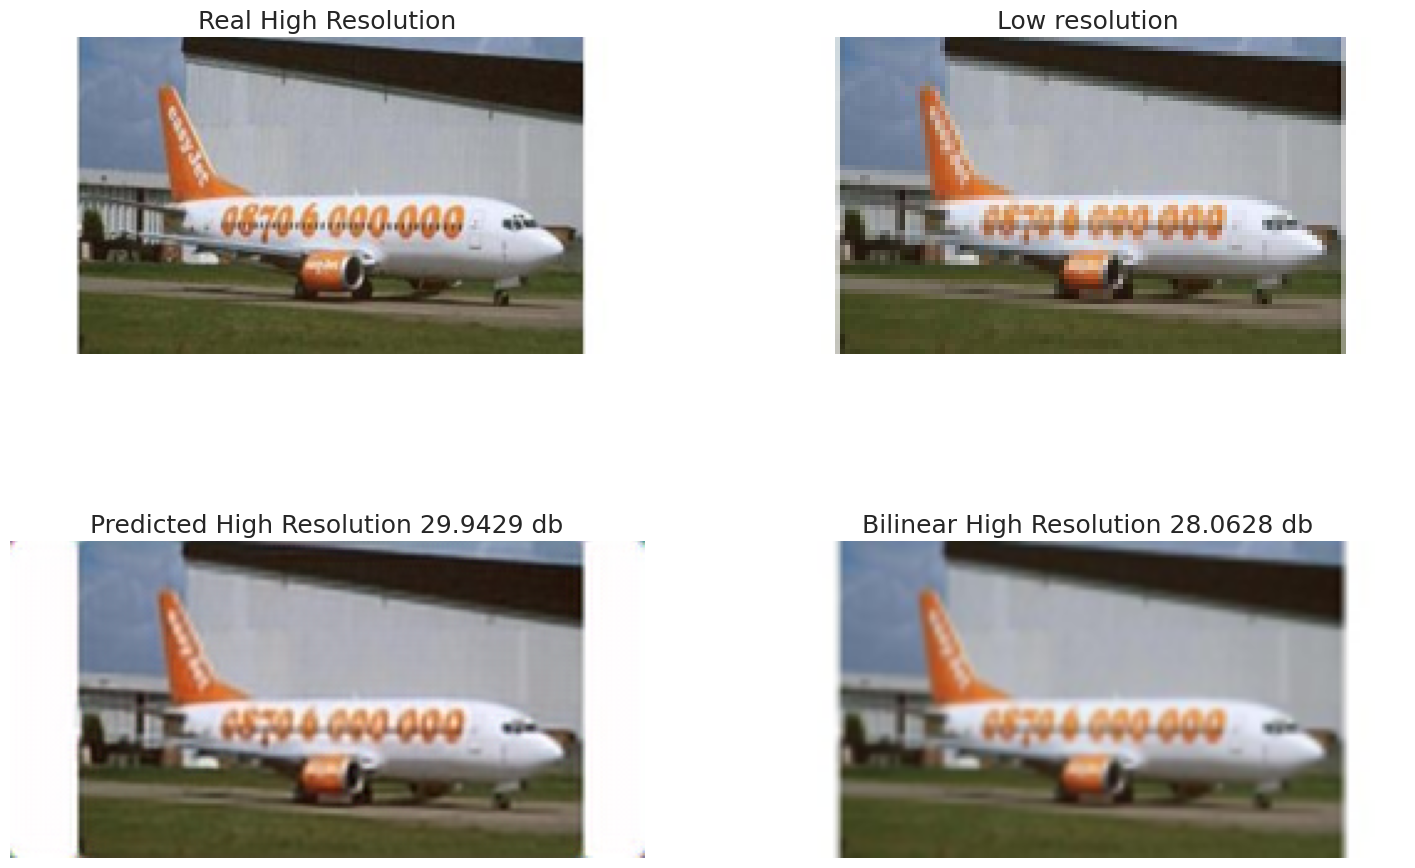
\includegraphics[width=\textwidth]{../images/validation.png}
\end{figure}
Continuing to train the best model for an additional 150 epochs using the combined training and validation set leads to the results shown in terms of loss and PSNR, as seen in Figure \ref{fig:loss} and Figure \ref{fig:db}. The classification of image quality levels as low, medium, and high based on PSNR values is a matter of convention and does not relate to resolution; it only indicates how much the generated image differs from the original.
\begin{figure}[H]
	\caption{L1 Loss}
	\centering
	\label{fig:loss}
	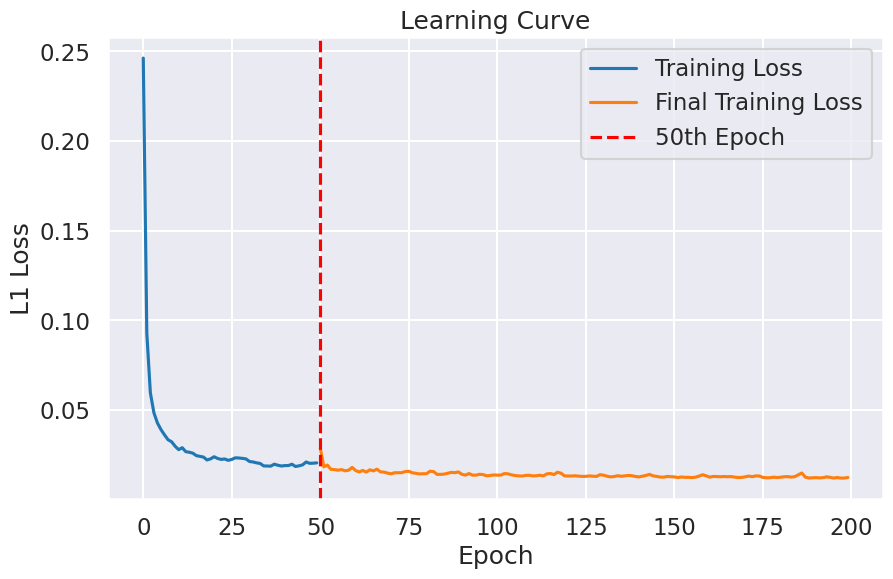
\includegraphics[width=\textwidth]{../images/loss.png}
\end{figure}

\begin{figure}[H]
	\caption{PSNR}
	\centering
	\label{fig:db}
	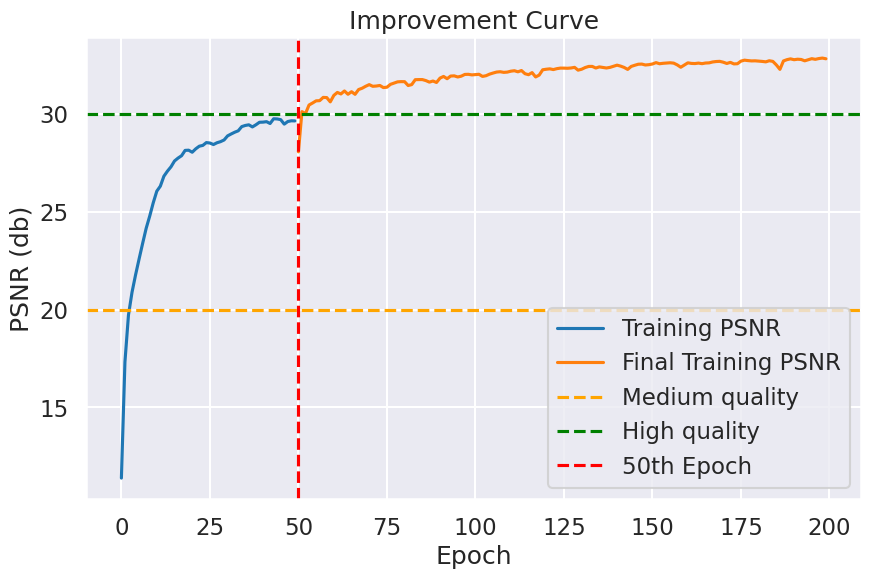
\includegraphics[width=\textwidth]{../images/db.png}
\end{figure}


	
\end{document}